%================
% Custom commands
%================
\thispagestyle{empty}
\newcommand{\degrees}{$^\circ$}
\setlength{\parindent}{12pt}

\begin{center}
	Potentially Useful Information
\end{center}

%\begin{center}
%Other fundamental principles:
%
%$\Delta \vec{L}_A = \vec{\tau}_{net,A} \Delta t$ \hspace*{30pt}  or \hspace*{30pt} $\dfrac{dL_{A}}{dt} = \vec{\tau}_{net,A}$ \\
%\end{center}
%
%\vspace{5pt}
%$\vec{L}_{trans,A} = \vec{r}_A \times \vec{p}$  (point particle) \hspace{1in}
%$\vec{\tau}_A = \vec{r}_A \times \vec{F}$\\

%\begin{center}
%Multiparticle systems:
%\end{center}
%
%\begin{tabbing}
%\hspace*{2.16in} \= \hspace*{2.16in} \= \kill    %% set tabs but don't print line
%
%$\vec{r}_{cm} = \dfrac{m_1 \vec{r}_1 + m_2 \vec{r}_2 + \ldots}{m_1 + m_2 + \ldots}$ \>
%$\vec{P}_{tot} \approx M_{tot} \vec{v}_{cm}$ ($v << c$) \>
%$K_{tot} = K_{trans} + K_{rel}$ \\
%\vspace{5pt}
%
%$K_{rel} = K_{rot} + K_{vib}$ \>
%$K_{trans} \approx \dfrac{1}{2}M_{tot} v_{cm}^2$  ($v << c$) \>
%\\

%$I = m_1 r_{1\bot}^2 + m_2 r_{2\bot}^2 + \ldots$ \\
%\vspace{5pt}
%
%$K_{rot} = \dfrac{L_{rot}^2}{2 I} = \dfrac{1}{2}I \omega^2$ \\
%\vspace{11pt}
%
%$\vec{L}_{trans,A} = \vec{r}_{cm,A} \times \vec{P}_{tot}$ \>
%$\vec{L}_{rot} = I \vec{\omega}$ \>
%$\vec{L}_A = \vec{L}_{trans,A} + \vec{L}_{rot}$ \\
%\end{tabbing}

%\begin{center}
%	Other physical quantities:
%\end{center}

\begin{tabular}{ll}
	%$\gamma \equiv \dfrac{1}{\sqrt{1-\left(\dfrac{\left|\vec{v}\right|}{c}\right)^2}}$ & $E^2 - \left(pc\right)^2 = \left(m c^2\right)^2$\\
	
	%\hspace{1in} \\  %% dummy row to make space below gamma
	
	$\vec F_{grav} = -G \dfrac{m_{1} m_{2}}{\left| \vec r \right|^2} \hat{r}$ &
	$U_{grav} = -G \dfrac{m_1 m_2}{\left| \vec r \right|}$ \\
	\vspace*{11pt}
	
	$\left| \vec F_{grav} \right| \approx m g$ near Earth's surface & $\Delta U_{grav} \approx mg \Delta y$ near Earth's surface\\
	\vspace*{5 pt}
	
	$\vec F_{elec} = \dfrac{1}{4 \pi \epsilon_{0}} \dfrac{q_{1} q_{2}}{\left| \vec r \right|^2} \hat{r}$  &
	$U_{elec} = \dfrac{1}{4 \pi \epsilon_0} \dfrac{q_1 q_2}{\left| \vec r \right|}$\\
	
	\vspace{5 pt}
	$\left| \vec F _{spring}\right| = k_{s} s$ opposite to the stretch \\
	%& $U_{spring} = \dfrac{1}{2}k_s s^2$ for ideal spring\\
	%
	%\vspace{10pt}
	%$U_i \approx \dfrac{1}{2}k_{si} s^2 - E_M$  approx. interatomic pot. energy \hspace{25pt} & $\Delta E_{thermal} = m C \Delta T$\\
	
\end{tabular}

%$E_N = -\dfrac{13.6 \mathrm{eV}}{N^2}$ where $N = 1,2,3 \ldots$ (Hydrogen atom energy levels)\\
%
%\vspace{5 pt}
%
%$E_N = N \hbar \omega_0 + E_0$ where $N = 0,1,2 \ldots$ and $\omega_0 = \sqrt{\dfrac{k_{si}}{m_a}}$ (Quantized oscillator energy levels)\\

\vspace{5 pt}
$\left| \left(\dfrac{d\vec p}{dt}\right)_\bot\right| = \dfrac{p v}{R} \approx \dfrac{m v^2}{R}$ (if $v << c$) where $R$ = radius of kissing circle\\

\begin{tabbing}
	\hspace*{2.16in} \= \hspace*{2.16in} \= \kill    %% set tabs but don't print line
	
	$\omega = \dfrac{2 \pi}{T}$\>
	$x = A\cos{\omega t}$ \>
	$\omega = \sqrt{\dfrac{k_s}{m}}$\\
	
	%\vspace*{11 pt}
	%$Y = \dfrac{F/A}{ \Delta L/L}$ (macro) \>
	%$Y = \dfrac{k_{si}}{d}$ (micro) \>
	%speed of sound $v = d \sqrt{\dfrac{k_{si}}{m_a}}$\\
\end{tabbing}

%\vspace{11 pt}

%\newpage
$\hat{f} = \left\langle \cos\theta_x, \cos\theta_y, \cos\theta_z \right\rangle$  unit vector from angles  \\

%\begin{center}
%Moment of intertia for rotation about indicated axis
%\vspace{11pt}
%
%\begin{tabular}{|c|c|c|c|} \hline
%
%\includegraphics{sphere.eps} & 
%\includegraphics{cyl1.eps} & 
%\includegraphics{cyl3.eps} & 
%\includegraphics{cyl2.eps} \\
%
%$I = \dfrac{2}{5} MR^2$ &
%$I = \dfrac{1}{2} MR^2$ &
%$I = \dfrac{1}{12} ML^2$ &
%$I = \dfrac{1}{12} ML^2 + \dfrac{1}{4} MR^2$\\ 
%
%  &  &  &   \\
%\hline
%\end{tabular}
%\end{center}

\vspace*{0.1 in}

%\begin{tabbing}
%\hspace*{2.16in} \= \hspace*{2.16in} \= \kill    %% set tabs but don't print line
%$\Omega = \dfrac{\left(q + N - 1\right)!}{q!\left(N-1\right)!}$ \>
%$S \equiv k \ln \Omega$ \>
%$\dfrac{1}{T} \equiv \dfrac{\partial{S}}{\partial{E}}$ \\
%$\Delta S = \dfrac{Q}{T}$ (small $Q$) \> 
%prob($E$) $\propto \Omega \left(E\right) e^{-\dfrac{E}{k T}}$ \\
%\end{tabbing}

\begin{tabular}{lcl}
	Constant & Symbol & Approximate Value \\ \hline
	Speed of light & $c$ & $3 \times 10^8$ m/s \\
	Gravitational constant & $G$ & $6.7 \times 10^{-11}$ N $\cdot \text{ m}^2$/$\text{kg}^2$\\
	Approx. grav field near Earth's surface & $g$ & $9.8$ N/kg\\
	Electron mass & $m_e$ & $9 \times 10^{-31}$ kg \\
	Proton mass & $m_p$ & $1.7 \times 10^{-27}$ kg \\
	Neutron mass & $m_n$ & $1.7 \times 10^{-27}$ kg \\
	Electric constant & $\dfrac{1}{4 \pi \epsilon_0}$ & $9 \times 10^9$ N $\cdot \text{ m}^2$/$\text{C}^2$\\
	Proton charge & $e$ & $1.6 \times 10^{-19}$ C \\
	Electron volt & 1 eV & $1.6 \times 10^{-19}$ J \\
	Avogadro's number & $N_A$ & $6.02 \times 10^{23}$ atoms/mol \\
	%    Plank's constant & $h$ & $6.6 \times 10^{-34}$ joule $\cdot$ second\\
	%    hbar $ = \dfrac{h}{2 \pi}$ & $\hbar$ & $1.05 \times 10^{-34}$ joule $\cdot$ second\\
	%    specific heat capacity of water & $C$ & $4.2$ J/kg\\
	%    Boltzmann constant & $k$ & $1.38 \times 10^{-23}$ J/K \\ 
	\hline
\end{tabular}

\vspace{.2in}
\begin{tabular} {lll|lll}
	milli & m & $1 \times 10^{-3}$ \hspace*{0.5in} & \hspace{0.5in} kilo & K & $1 \times 10^{3}$\\
	micro & $\mu$ & $1 \times 10^{-6}$ &  \hspace{0.5in} mega & M & $1 \times 10^{6}$\\
	nano & n &$1 \times 10^{-9}$ &  \hspace{0.5in} giga & G & $1 \times 10^{9}$\\
	pico & p & $1 \times 10^{-12}$ &  \hspace{0.5in} tera & T & $1 \times 10^{12}$ \\
\end{tabular}


\begin{center}
	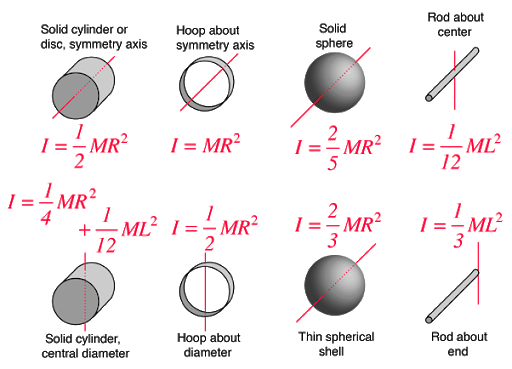
\includegraphics[width=9cm]{moments_of_inertia.png}
\end{center}